%\documentclass[12pt,a4paper]{article}

\setlength{\parindent}{0.1 in}
%\setlength{\parskip}{0.1 in}
\setlength{\oddsidemargin}{0.25 in}
\setlength{\evensidemargin}{-0.25 in}
\setlength{\topmargin}{-0.5 in}
\setlength{\textwidth}{7.0 in}
\setlength{\textheight}{9.5 in}
\setlength{\headsep}{0.45 in}

%\usepackage[fleqn]{amsmath}
%\usepackage{amsfonts,graphicx}
\usepackage{amsmath,amsfonts,graphicx}
\usepackage[fleqn]{mathtools}
\usepackage{setspace}
\usepackage[colorlinks=false, pdfborder={0 0 0}]{hyperref}
\usepackage[nottoc]{tocbibind}
\usepackage{tocloft}
\usepackage[outermargin=2 in]{geometry}
\usepackage{scrextend}
\usepackage{tensor}
\usepackage{cancel}
\usepackage{slashed}


%Adding `Appendix' to the appendices
\usepackage[toc,page]{appendix}

%Add a bullet point to description items
\usepackage{enumitem}

%Mathematics
\usepackage{braket}
\usepackage{ulem}
\usepackage{xcolor}
\usepackage[font={small,it}]{caption}

\bibliographystyle{unsrt}

% Packages that Gavin uses
\usepackage{url}
\usepackage[font=footnotesize]{caption}
\usepackage[font=footnotesize]{subcaption}
\usepackage[]{microtype}
\usepackage{balance}
\usepackage{cite}
\usepackage{lmodern}
\usepackage[T1]{fontenc}
\usepackage{doi}

% Nice typesetting of SI units
\usepackage{siunitx}
\sisetup{range-phrase=--}
\sisetup{separate-uncertainty = true}

% SImons packages
\usepackage{float}





%
%   This file is part of the APS files in the REVTeX 4.1 distribution.
%   Version 4.1r of REVTeX, August 2010
%
%   Copyright (c) 2009, 2010 The American Physical Society.
%
%   See the REVTeX 4 README file for restrictions and more information.
%
% TeX'ing this file requires that you have AMS-LaTeX 2.0 installed
% as well as the rest of the prerequisites for REVTeX 4.1
%
% See the REVTeX 4 README file
% It also requires running BibTeX. The commands are as follows:
%
%  1)  latex apssamp.tex
%  2)  bibtex apssamp
%  3)  latex apssamp.tex
%  4)  latex apssamp.tex
%
\documentclass[%
 reprint,
%superscriptaddress,
%groupedaddress,
%unsortedaddress,
%runinaddress,
%frontmatterverbose, 
%preprint,
%showpacs,preprintnumbers,
%nofootinbib,
%nobibnotes,
%bibnotes,
 amsmath,amssymb,
 aps,
%pra,
%prb,
%rmp,
%prstab,
%prstper,
%floatfix,
]{revtex4-1}

\usepackage{graphicx}% Include figure files
\usepackage{dcolumn}% Align table columns on decimal point
\usepackage{bm}% bold math
%\usepackage{hyperref}% add hypertext capabilities
%\usepackage[mathlines]{lineno}% Enable numbering of text and display math
%\linenumbers\relax % Commence numbering lines

%\usepackage[showframe,%Uncomment any one of the following lines to test 
%%scale=0.7, marginratio={1:1, 2:3}, ignoreall,% default settings
%%text={7in,10in},centering,
%%margin=1.5in,
%%total={6.5in,8.75in}, top=1.2in, left=0.9in, includefoot,
%%height=10in,a5paper,hmargin={3cm,0.8in},
%]{geometry}


%Mathematics
\usepackage{braket}
\usepackage{ulem}
\usepackage{xcolor}
\usepackage[font={small,it}]{caption}
%New commands
%Maths
\newcommand{\beq}{\begin{equation}}
\newcommand{\eeq}{\end{equation}}
\newcommand{\bea}{\begin{align}}
\newcommand{\eea}{\end{align}}
\newcommand{\p}{\partial}
\newcommand{\trace}[1]{\mathrm{Tr}\left[#1 \right]}
\newcommand{\ptrace}[2]{\mathrm{Tr}_{#1} \left[ #2 \right]}
\newcommand{\bpmat}{\begin{pmatrix}}
\newcommand{\epmat}{\end{pmatrix}}
\newcommand{\vv}[1]{\mathbf{#1}}
\newcommand{\mat}[1]{\uuline{#1}}
\newcommand{\norm}[1]{\| #1 \|}
\newcommand{\op}[1]{\mathbb{#1}}
\newcommand{\vhat}[1]{\hat{\vv{#1}}}

%Renewed commands, in order for them to take arguments with automatically adjusted brackets 
\renewcommand{\dim}[1]{\mathrm{dim}\left( #1\right)}
\renewcommand{\det}[1]{\mathrm{det} \left( #1 \right)}
\renewcommand{\exp}[1] {\mathrm{exp} \left[ #1 \right]}


%\mathbb Letters
\newcommand{\identity}{\mathbb{I}}
\newcommand{\inreal}{\mathbb{R}}
\newcommand{\incomplex}{\mathbb{C}}

%Redefine Braket
\renewcommand{\braket}[1]{\left\langle #1 \right\rangle}

%Integration
\newcommand{\intd} {\mathrm{d}}

%Operators
\newcommand{\phihat}{\hat{\phi}}
\newcommand{\xhat}{\hat{x}}
\newcommand{\phat}{\hat{p}}
\newcommand{\Dhat}{\hat{D}}
\newcommand{\Hhat}{\hat{H}}
\newcommand{\ahat}{\hat{a}}
\newcommand{\bhat}{\hat{b}}
\newcommand{\chat}{\hat{c}}
\newcommand{\Phihat}{\hat{\Phi}}

%Channels
\newcommand{\channel}[3]{\mathcal{#1}^{#2 \rightarrow #3}}


%Caligraphy letters
\newcommand{\cl}[1]{\mathcal{#1}}
\newcommand{\Hilbert}{\mathcal{H}}
\newcommand{\calN}{\mathcal{N}}
\newcommand{\Lag}{\mathcal{L}}
\newcommand{\calD}{\mathcal{D}}


%Pauli
\newcommand{\Xhat}{\hat{X}}
\newcommand{\Yhat}{\hat{Y}}
\newcommand{\Zhat}{\hat{Z}}
\newcommand{\PauliX}{\bpmat 0 & 1 \\ 1 & 0 \epmat}
\newcommand{\PauliZ} {\bpmat 1 & 0 \\ 0 & -1\epmat}



%Gell-Mann matrices
\newcommand{\GMone} {\bpmat 0 & 1 & 0 \\ 1 & 0 & 0 \\ 0 & 0 & 0 \epmat }
\newcommand{\GMsix}{\bpmat 0 & 0 & 0 \\ 0 & 0 & 1\\ 0 & 1 & 0\epmat}

%Density matrices
\newcommand{\rhotwo}{\bpmat 1 & e^{-it} \\ e^{it} & 1 \epmat}
\newcommand{\rhothree} {\bpmat 1 & e^{it} & e^{2it} \\
e^{-it} & 1 & e^{it} \\
e^{-2it} & e^{-it} & 1 \epmat}



%Misc
\def\dbar{{\mathchar'26\mkern-12mu d}} %a $d$ with a bar through its stem


\newcommand{\eq}[1]{$#1$}

%Undertilded quantities
\newcommand{\tildeq}{\underset{^\sim}q}
\newcommand{\tildep}{\underset{^\sim}p}

%Curly letters
\newcommand{\calE}{\mathcal{E}}

\newcommand{\Nhat}{\hat{N}}

%Wave vector shortening
\newcommand{\kvec}{\vv{k}}














% Packages that Gavin uses
\usepackage{url}
\usepackage[font=footnotesize]{caption}
\usepackage[font=footnotesize]{subcaption}
\usepackage[]{microtype}
\usepackage{balance}
%\usepackage{cite}
\usepackage{lmodern}
\usepackage[T1]{fontenc}
%\usepackage{doi}


% Nice typesetting of SI units
\usepackage{siunitx}
\sisetup{range-phrase=--}
\sisetup{separate-uncertainty = true}

% SImons packages
\usepackage{float}


\begin{document}

\preprint{APS/123-QED}

\title{Simulating an implementation of the surface code in silicon }% Force line breaks with \\
\thanks{The authors would like to thank Dan Browne and John Morton for fruitful discussions. }%

\author{Gavin Dold}
\author{Sofia Qvarfort}
% \email{Second.Author@institution.edu}
 
\author{Simon Schaal}
 %\email{Second.Author@institution.edu}
\affiliation{% 
Centre for Doctoral Training in Delivering Quantum Technologies
Department of Physics and Astronomy, University College London
}%'


%\collaboration{CLEO Collaboration}%\noaffiliation

\date{\today}% It is always \today, today,
             %  but any date may be explicitly specified

\begin{abstract}
We simulate a simple system consisting of one probe qubit and four data qubits as proposed in \cite{the paper} and implement errors such as dephasing, dopant displacement, and path jitter to the full stabiliser measurement cycle. 
\end{abstract}

\pacs{Valid PACS appear here}% PACS, the Physics and Astronomy
                             % Classification Scheme.
%\keywords{Suggested keywords}%Use showkeys class option if keyword
                              %display desired
\maketitle

%\tableofcontents

\section{Introduction} \label{sec:Introduction}





Due to its usefulness in the semiconductor industry, silicon is one of the most well-studied and well-udnerstood materials used for classical computers. For quantum computers, a plethora of qubit materials are still being investigated, but it has proven difficult to use silicon due to its .... [insert something]. 

There has been a recent proposal to make use of dopants in silicon to act as qubits \cite{the paper} to implement a version of the surface code. 


We have simulated a probe qubit interacting with four data qubits. The probe qubit is performing a circular orbit $40$ nm above the data qubits, and in this document we will document the effect of various errors. These errors include dephasing, dopan placement uncertainties and a path jitter. 

\subsection{The proposal}
Let us first take a closer look at the scheme proposed in \cite{the paper}. The data qubits are dopants placed in silicon placed in a square pattern using the best dopant placement techniques available, which currently stand at [insert some error value and cite it]. To perform the stabiliser measurements, a probe qubit of a different dopant species is placed on a mobile slab above the data qubits. Each probe qubit performs a stabiliser measurement on four data qubits, a procedure which is performed by physically moving the overhead slab with the probe qubits. 

Some differences in physical parameters are required. 

\subsection{Spin species}

\begin{table}
\begin{tabular}{ccccccccc}
	& $T_1^e$ & $T_2^{e*}$ & $T_2^e$ & $T_{2, decoupl}^e$ & $T_1^N$ & $T_2^{N*}$ & $T_2^N$ & $T_{2, decoupl.}^N$\\ \hline
P (nat. Si, SET) \cite{Pla2012}& $0.7\, $s & $55\, $ns  & $206\, \mu$s & $410\, \mu$s &  & & \\
P (puri. Si, SET) \cite{Muhonen2014}&  & $160\, \mu$s  & $1\, $ms & $560\, $ms & & $500\, \mu$s & $1.75\, $s & $35.6\, $s \\
Bi (puri. Si, CT) \cite{Wolfowicz2013} & $9\, $s &  & $2.7\, $s && && &\\
NV (puri. C, RT) \cite{Balasubramanian2009,Bar-Gill2013} & & & $1.8\, $ms & $3.3\, $ms && &&\\
NV (puri. C, $77\, $K) \cite{Bar-Gill2013} & & &  & $0.6\, $s && &&\\
SiC ($20\, $K) \cite{Christle2014} & & $1.1\, \mu$s & $1.2\, $ms & && && \\
SiC (RT) \cite{Koehl2011} & $185\, \mu$s & $214\, $ns & $40\, \mu$s &  & & && \\
\hline
\end{tabular} 
\label{lala}
\caption{\cite{Pla2012,Muhonen2014}: high field >1T low temp mK. Even good coherenc ebeing close to suurface.}
\end{table}

Donors deep in bulk show longer coherence times $T_2^e=2\, $s \cite{Tyryshkin2011} not applicable for us.


\section{The Simulation}
In this section, we will describe how we go about simulating the interaction between the probe qubit and the data qubit. The interaction is governed by the following Hamiltonian:

\begin{equation}
H = \mu_B B( g_1 \sigma_1^Z + g_2 \sigma_2^Z) + \frac{J}{r^3} ( \mathbf{\sigma_1} \cdot \mathbf{\sigma_2} - 3 ( \hat{\mathbf{r}} \cdot \mathbf{\sigma_1}) ( \hat{\mathbf{r}}\cdot \mathbf{\sigma_2}))
\end{equation}
The effect of this Hamiltonian is to evolve the probe qubit in a particular direction depending on the state of the data qubit. By initialising the probe qubit in the $\ket{+}$ state, the final parity measurement will entail finding the probe qubit in either the $\ket{+}$ state (even parity) or in the $\ket{-}$ state. This can be understood by the fact that each data qubit imparts a $\frac{\pi}{2}$ phase in 

\subsection{Finding the correct evolution time}
The speed of the simulation is set by the total time it takes to complete one full cycle. We want the accumulated phase for an even parity measurement to reach $2\pi$ exactly. The plot in Figure \ref{fig:plot} shows the accumulated phase as a function of evolution time. 





\begin{figure}[H]
	\centering
	\begin{subfigure}[t]{0.49\textwidth}
		\centering
		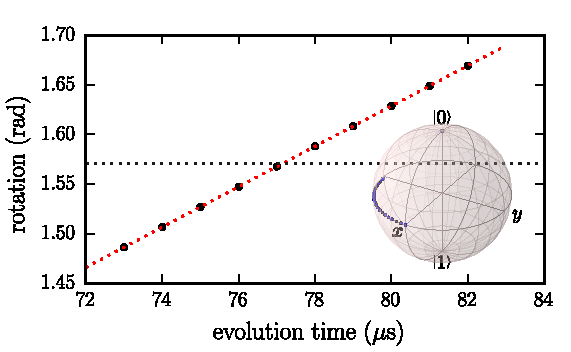
\includegraphics[width=\linewidth]{abrupt_find_tau/abrupt_find_tau_full.pdf}
		\caption{}
		\label{fig:abrupt_tau}
	\end{subfigure}
	\begin{subfigure}[t]{0.49\textwidth}
		\centering
		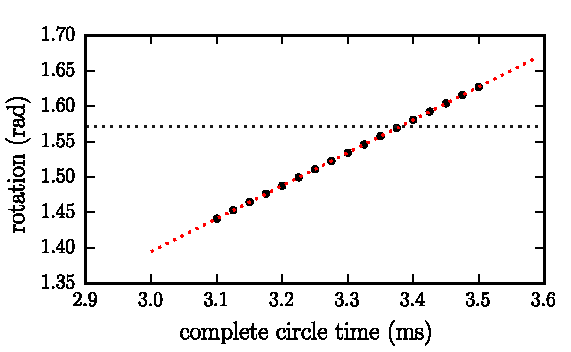
\includegraphics[width=\linewidth]{circular_find_tau/circle_find_tau.pdf}
		\caption{}
		\label{fig:circ_tau}
	\end{subfigure}
	\label{fig:find_tau}
	\caption{Finding the correct evolution time. (a) abrupt. (b) circular}
\end{figure}


\begin{figure}[H]
	\centering
	\begin{subfigure}[t]{0.30\textwidth}
		\centering
		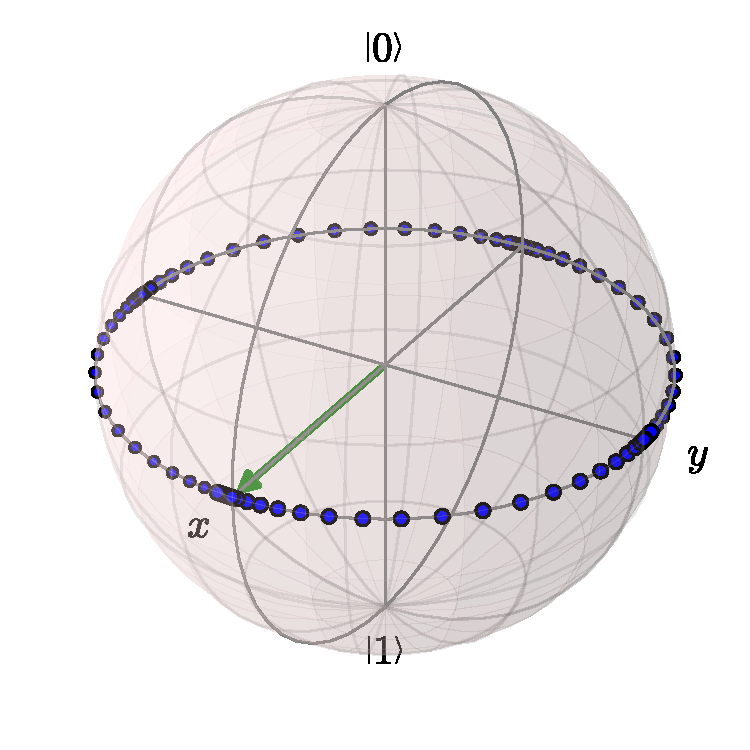
\includegraphics[width=\linewidth]{Figures/notodd.pdf}
		\caption{}
		\label{fig:notodd}
	\end{subfigure}
	\begin{subfigure}[t]{0.30\textwidth}
		\centering
		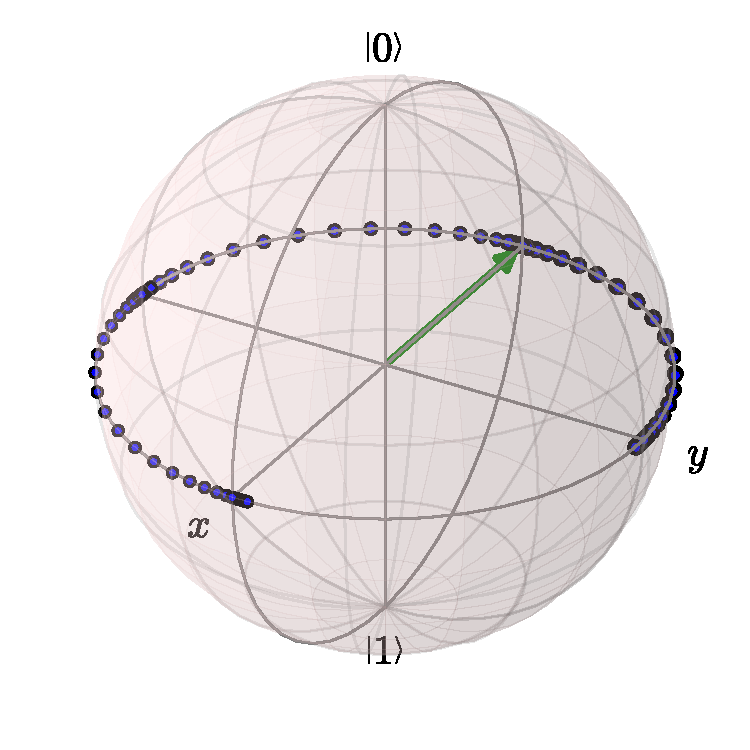
\includegraphics[width=\linewidth]{Figures/odd.pdf}
		\caption{}
		\label{fig:odd}
	\end{subfigure}
	\label{fig:paritymeas}
	\caption{Example of parity measurement for the circular motion. (a) no error in data qubits. plus state is final state. (b) error on last qubit. minus state is final state.}
\end{figure}





\subsection{Dephasing}
In this section, we present results from simulations of the Lindblad master equation where a dephasing channel is turned on. This channel contains the Lindblad operator
\beq
L  = \sqrt{\Gamma} \sigma_z
\eeq

where $\Gamma$ is the dephasing parameter. $\Gamma$ can also be written as $1/\tau$ where $\tau$ is the dephasing time. We evolve the system under the Lindblad master equation for an odd number of errors. In this simulation, the error is a bit-flip error on the fourth data qubit.  As a result, the probe qubit `backtracks'  during the last quarter of the run such that its final phase ends up at $\phi = \pi$. 

In Figure \ref{fig:BlochsphereDephasing}, we see the effect of a small dephasing coefficient (100) whereas in Figure \ref{fig:BlochsphereDephasing2} we see the effect of larger dephasing (500). Note that the dephasing happens primarily as the interaction between the probe qubit and the data qubit is weak, where the phase of the probe qubit doesn't evolve. 



\begin{figure}[h]
  \centering
    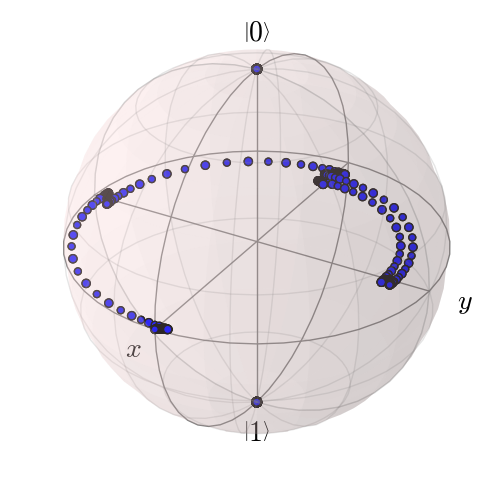
\includegraphics[width=0.5\textwidth]{Figures/Circ_orbit_odd_100_dephasing.png}
      \caption{The states of the probe and data qubits plotted in the Bloch sphere with a dephasing parameter of 100, which translates to a dephasing time of 10 ms. The phase of the probe qubit is not affected since no relaxation or excitation is taking place. The effect can however be seen in the probability of measuring the probe qubit in the $\ket{+}$ or $\ket{-}$ state. For complete dephasing, the probe qubit will become the maximally mixed state and the measurement outcomes are completely random. The states of the probe and data qubits plotted in the Bloch sphere with a dephasing parameter of 100, which translates to a dephasing time of 10 ms.}
      \label{fig:BlochsphereDephasing}
      
\end{figure}




\begin{figure}[!h]
  \centering
    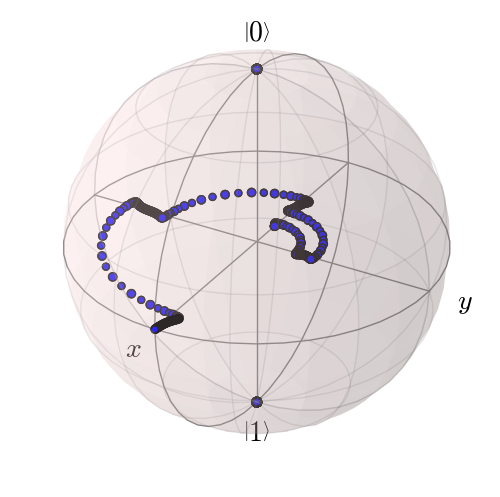
\includegraphics[width=0.5\textwidth]{Figures/Circ_orbit_odd_500_dephasing.png}
      \caption{The states of the probe and data qubits plotted in the Bloch sphere with a dephasing parameter of 500, which translates to a dephasing time of 2 ms. The strong dephasing causes the probe qubit state to drift quickly towards the maximally mixed state. }
      \label{fig:BlochsphereDephasing2}
\end{figure}

In Figure \ref{fig:phaseplot} we see the effect of dephasing on the probability of measuring the correct value of the probe qubit. Since there is an odd number of errors, we want the probe qubit to end up in the $\ket{-}$ state. However, the dephasing will cause the probe qubit to become a mixed state $\rho$, which means that there is a non-zero probability of measuring $\ket{+} $ instead of $\ket{-}$. For complete dephasing, the probe qubit becomes a mixed state which has a 50--50\% chance of measuring either state. 

\begin{figure}[!ht]
	\centering
	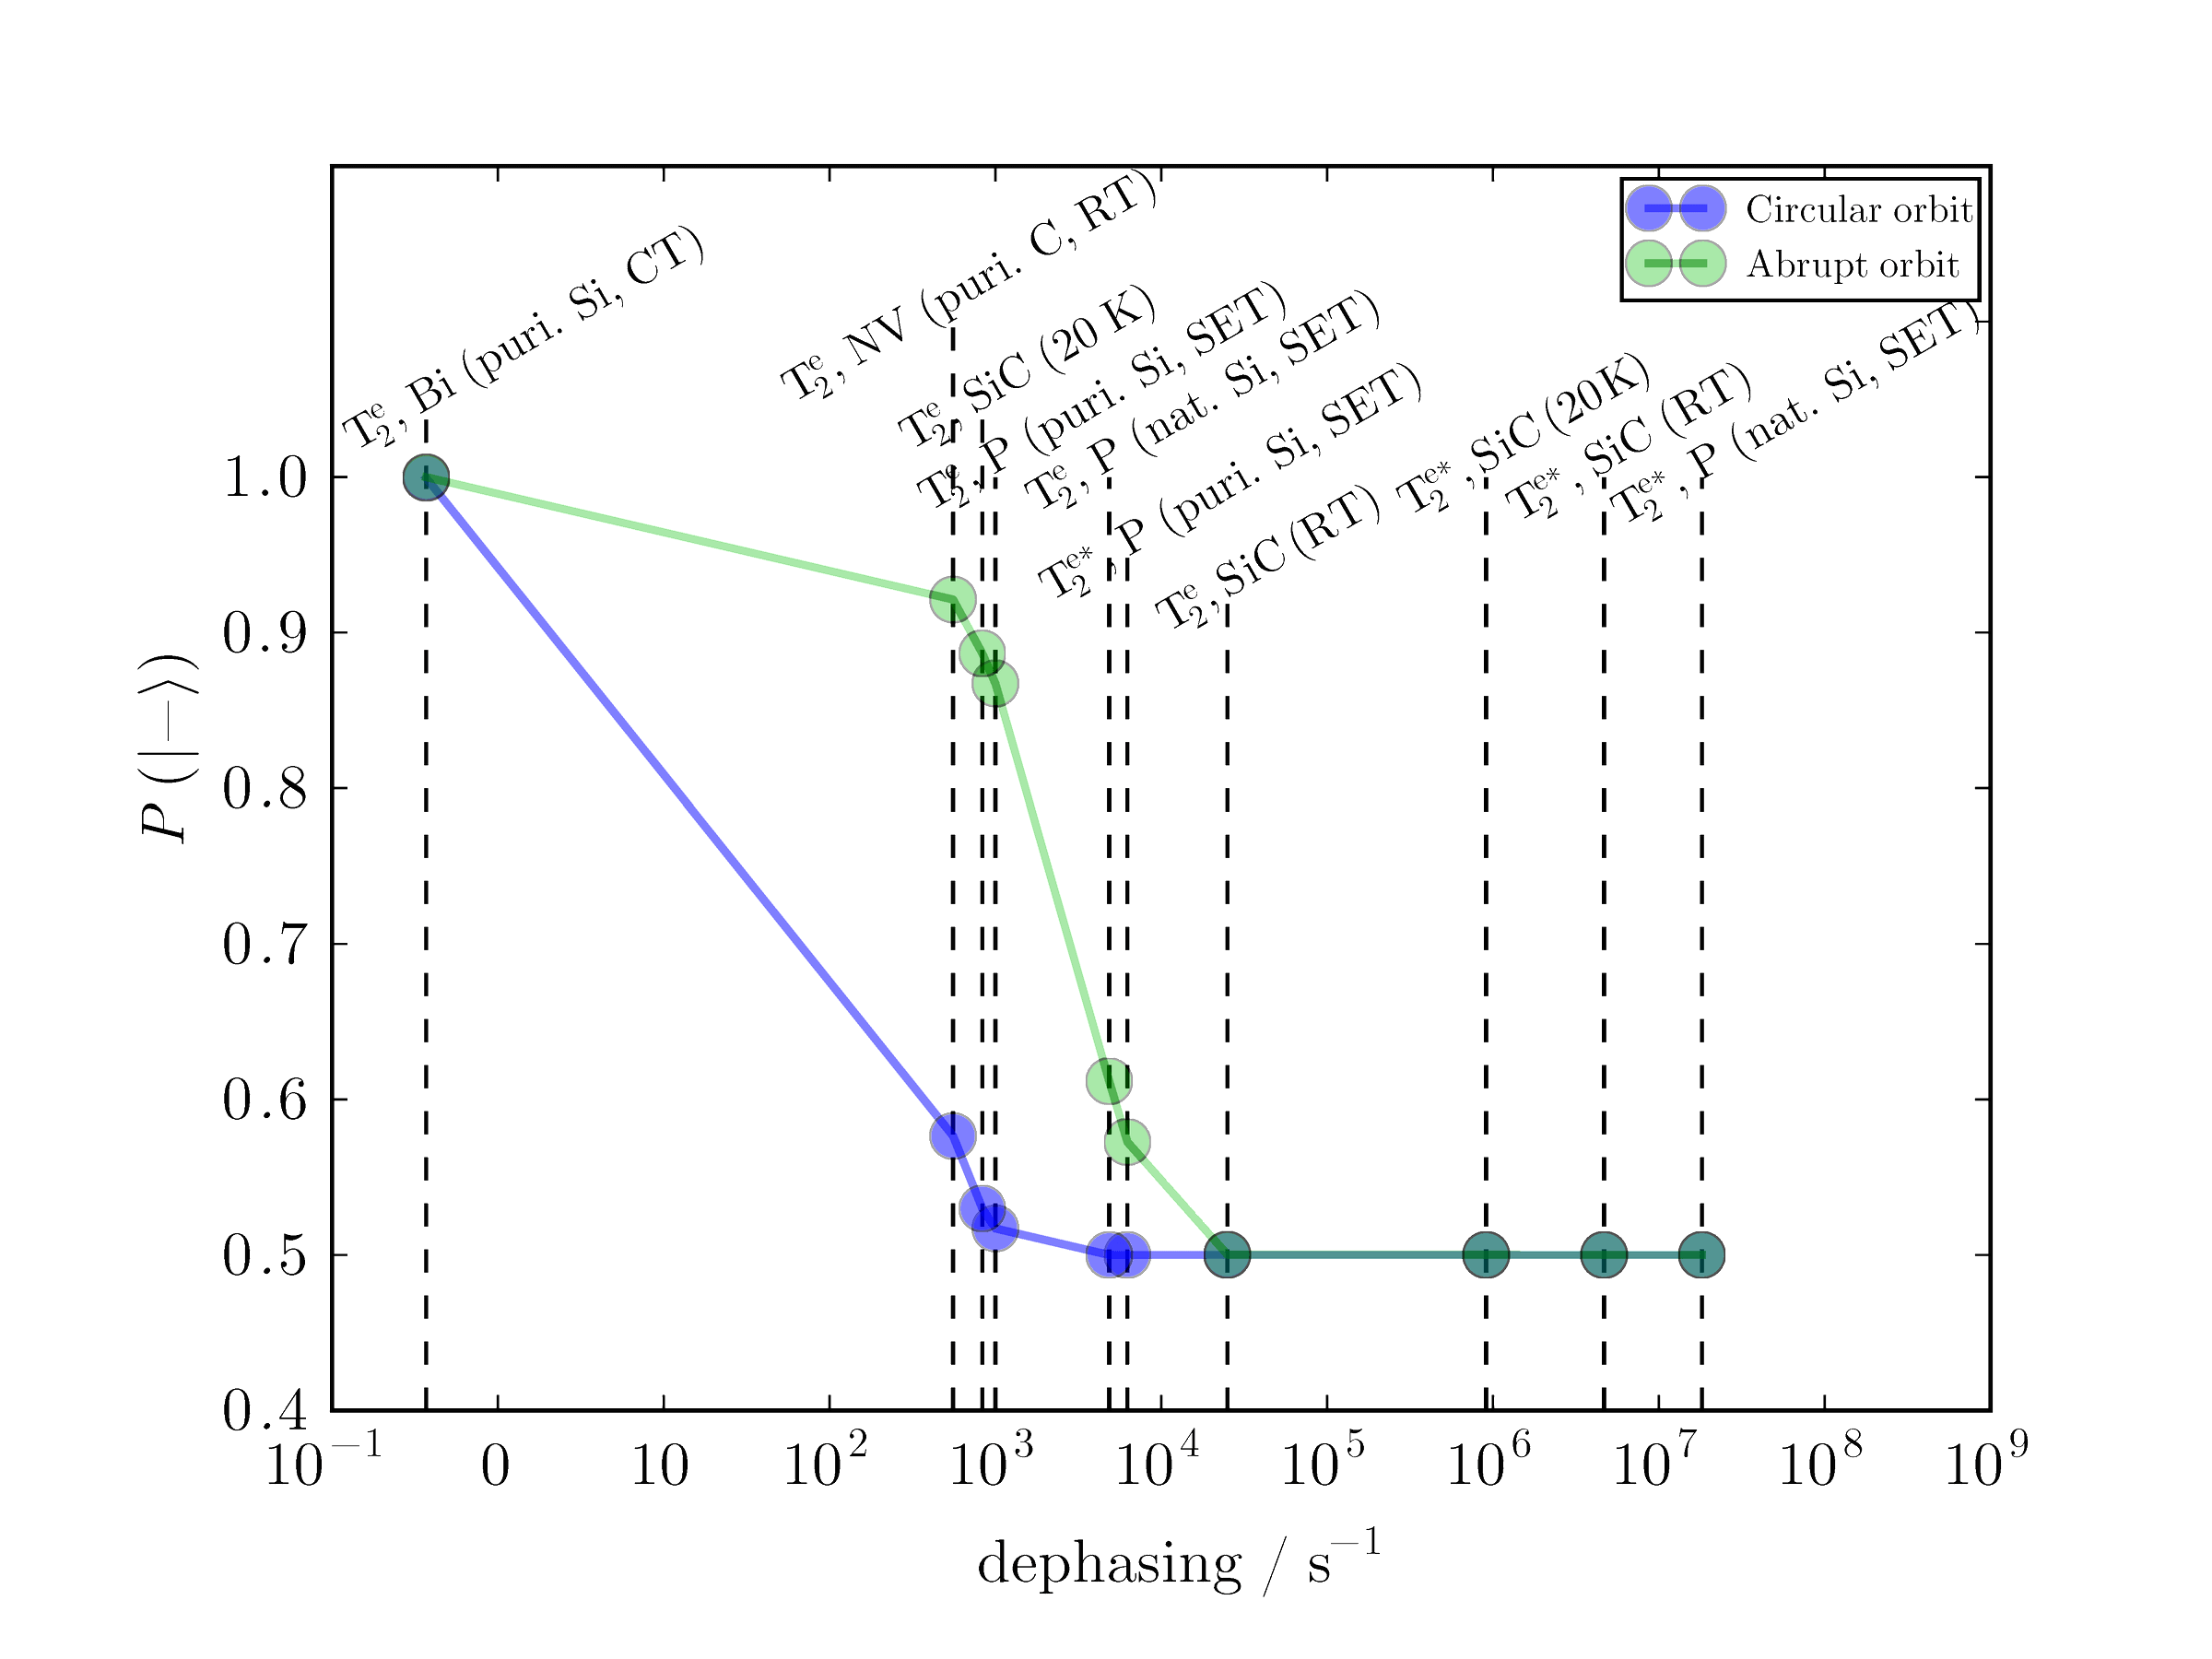
\includegraphics[width=\textwidth]{Figures/phase_graph.png}
		\caption{A graph showing the relationship between the dephasing parameter $\Gamma$ and the probability $P(\ket{-})$ of measuring the probe qubit in the $\ket{-}$ state. In this simulation, one of the data qubits have undergone a bit-flip error. As the dephasing parameter increases, the probe qubit moves towards the maximally mixed state and the probability of measuring $\ket{-}$ goes towards 0.5. The dephasing parameter for Bismuth as a material for the probe qubit has been market in the graph.}
		\label{fig:phaseplot}
\end{figure}


In Figure \ref{fig:phaseplot}, we have market the data-point for dephasing corresponding to the decoherence time for Bismuth, which is one of the proposed donor types for the probe qubit. The decoherence time of bismuth is \SI{2.7}{\second} \cite{Wolfowicz2013}, which leads to a dephasing parameter of \SI{0.37}{\per\second}. 


It should be noted that the Bismuth dephasing time of 2.7 s can only be obtained by applying advanced Hahn echo readout methods. Whereas it is cumbersome, this technique is not beyond the capabilities of modern experiments. 

%\clearpage
\subsection{Data qubit displacement}
The effect of displacement of the data qubits from the ideal was investigated. Ideally the data qubits would be in a square lattice of spins precisely $D = \SI{400}{\nano\metre}$ apart, but due to inaccuracies in dopant spin placement each qubit will have small displacements from the ideal lattice position.

This is modelled by generating a uniform random displacement within a given pillbox $xy$-radius and $z$-height. Simulations from the original paper show $\textrm{radius} = \textrm{height} = \SI{6}{\nano\metre}$ to be a threshold for this scheme. The phase accumulated over 25 runs for this pillbox size is plotted as a histogram in fig.\@ \ref{fig:DisplacementPhaseHistogram}, showing a maximum phase error of $\tfrac{\pi}{4}$ for these runs. 



The effect of displacements in the $x$-$y$ plane and the $z$-axis are significantly different in magnitudes, due to the $\tfrac{1}{d^3}$ term in the Hamiltonian being most strongly affected by $z$ displacements. This effect was investigated by artificially setting displacements in these directions.

Fig.\@ \ref{fig:zoffset} shows changes in accumulated phase due to $z$-displacements. The first 2 qubits are displaced \SI{4}{\nano\metre} down, slowing the evolution and giving a noticeable phase error after half a cycle. However, qubit 4 is displaced \SI{3}{\nano\metre} upwards, reducing $d$ and resulting in faster evolution. The effect is a small phase error from the ideal $2\pi$.

Fig.\@ \ref{fig:inwarddisplacement} shows the effect of displacements in the $x$-$y$ plane. For this run, all data qubits were displaced \SI{10}{\nano\metre} inwards with respect to the circular motion. The phase error on each individual qubit is then less than that produced by the \SI{3}{\nano\metre} $z$-displacement of fig.\@ \ref{fig:zoffset}, showing the smaller sensitivity to displacement in the $x$-$y$ plane, though the overall error after all 4 qubits is greater as in the $z$-direction, +$z$ and --$z$ errors cancel out somewhat, whereas $xy$ displacement errors will always slow the evolution.

\begin{figure}[h]
	\centering
	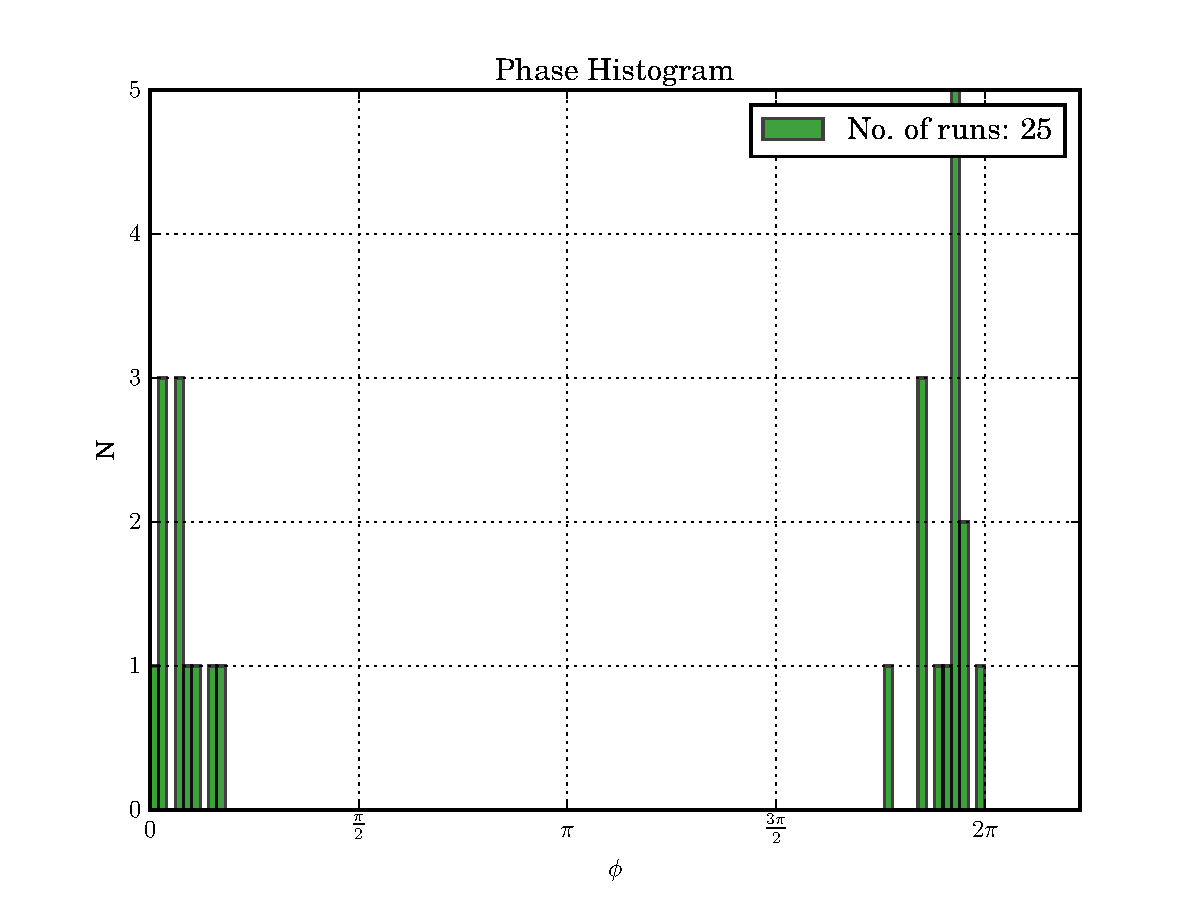
\includegraphics[width=\textwidth]{Figures/Displacement_phase_histogram.pdf}	
	\caption{Phase errors over 25 runs as a result of randomly generated data qubit displacements within a pillbox of half-height \SI{3}{\nano\metre} and radius \SI{6}{\nano\metre}. These values are a threshold for the proposed scheme.}
	\label{fig:DisplacementPhaseHistogram}
\end{figure}



\begin{figure}
	\centering
	\caption{Phase errors as a result of misplaced data qubits.}
	\begin{subfigure}[t]{\textwidth}
		\centering
		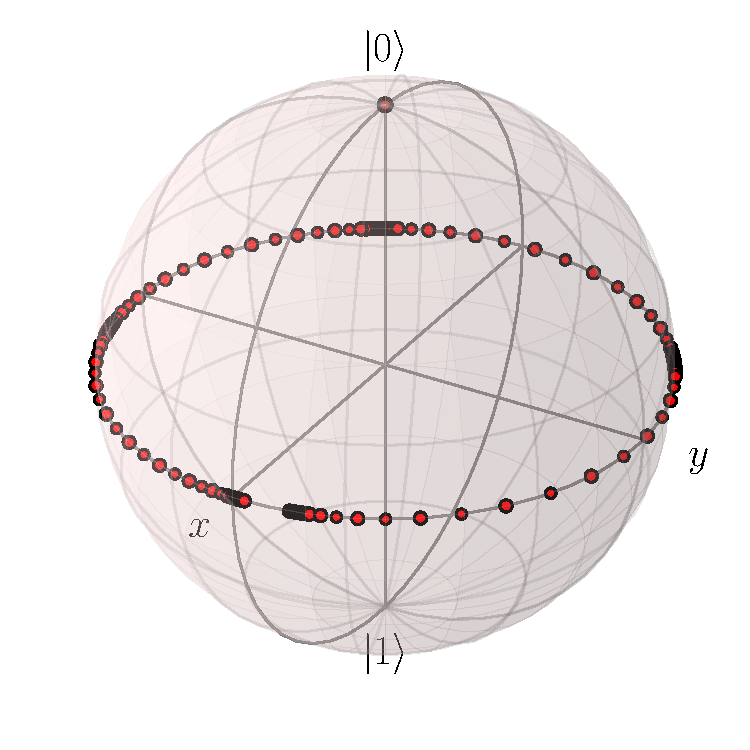
\includegraphics[width=0.7\textwidth]{figures/z_offset.pdf}
		\caption{Evolution of probe qubit with data qubit displacement in the Z direction. 1st and 2nd qubits are displaced \SI{4}{\nano\metre} down, slowing the evolution, the 4th is displaced \SI{3}{\nano\metre} up with a resultant increase in phase accumulated. The overall deviation from $2\pi$ is small as a result.}
		\label{fig:zoffset}
	\end{subfigure}
	\begin{subfigure}[t]{\textwidth}
		\centering
		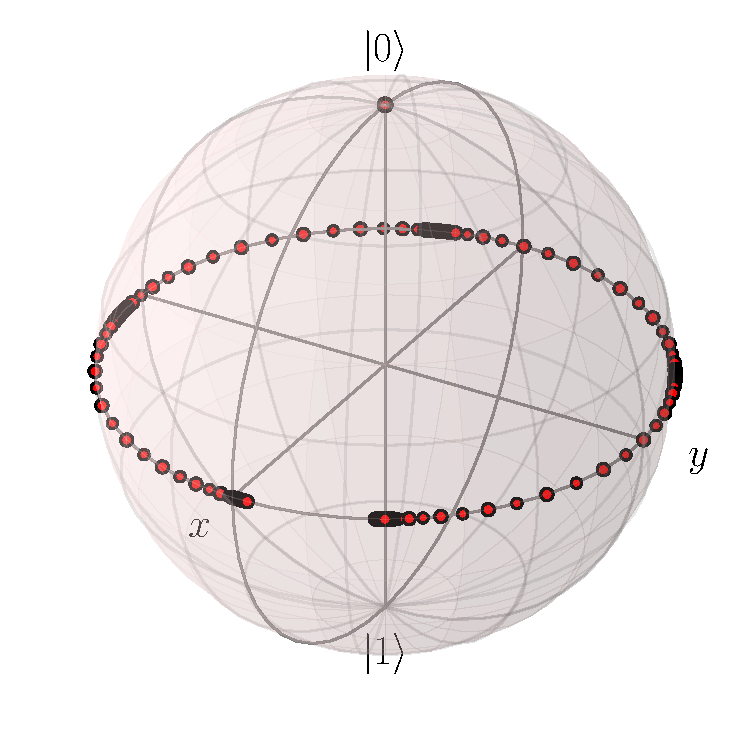
\includegraphics[width=0.7\textwidth]{figures/10nm_displacement_inward.pdf}
		\caption{Phase accumulated when all 4 data qubits are displaced \SI{10}{\nano\metre} towards the centre of the circle. Other directions of \SI{10}{\nano\metre} displacements result in similar phase deviations.}
		\label{fig:inwarddisplacement}
	\end{subfigure}
	\label{fig:overall_displacement}
\end{figure}

\subsection{Twirling}

\subsection{Path Jitter}
The final error that we introduce and simulate is jitter in the path taken by the probe qubits. The precision provided by modern MEMS control structures is about 1 nm \cite{MEMS precision}, 

It was found that adding just a random jitter to the path introduced jumps which the solver could not handle very well. Instead, we overlay a sinusoidal motion over the circular motion, effectively causing a periodic deviation from the perfect path. We introduced a random element in the starting phase and amplitude [check this!] 


\begin{figure}[H]
	\centering
	\begin{subfigure}[t]{0.49\textwidth}
		\centering
		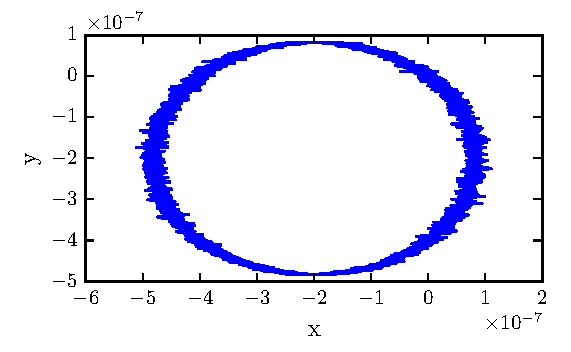
\includegraphics[width=\linewidth]{Figures/xjit.pdf}
		\caption{}
		\label{fig:xjit}
	\end{subfigure}
	\begin{subfigure}[t]{0.49\textwidth}
		\centering
		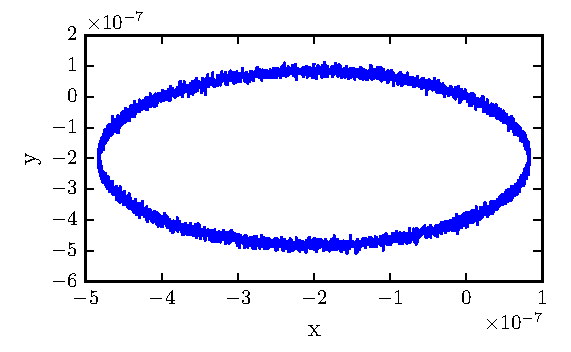
\includegraphics[width=\linewidth]{Figures/yjit.pdf}
		\caption{}
		\label{fig:yjit}
	\end{subfigure}
	\begin{subfigure}[t]{0.49\textwidth}
		\centering
		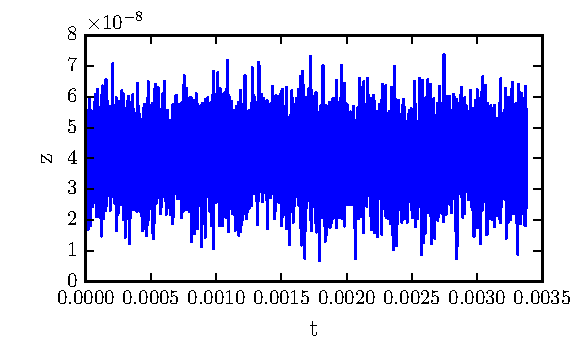
\includegraphics[width=\linewidth]{Figures/zjit.pdf}
		\caption{}
		\label{fig:zjit}
	\end{subfigure}
	\label{fig:paritymeas}
	\caption{Making sure path jitter works as expected. (a) xjit. (b) yjit. (c) zjit.}
\end{figure}




\section{Conclusions and outlook }
In this report, we have presented the results obtained from simulating the interaction between one probe qubit and four data qubits as in the proposed scheme in \cite{the paper}. 




\iffalse 
\begin{itemize}
\item Simulate path jitter
\item Combine errors
\item Find phase error $\phi_e$ for 1/4 of the run
\item Investigate how errors `stack' (e.g. is $\phi_e(2\pi)$ for a full circle equal to $4\phi_e(\pi/2)$?
\item Extract realistic physical parameters for the magnetic field $B$
\item Check effect of flip-flopping for different $\Delta$
\item Test different donor species ($g_1$, $g_2$
\item Sinusoidal motion in the $z$-direction (dip down over data qubits)
\end{itemize}
\fi




\bibliography{papers}

\end{document}
